\section{Sample Spaces and Probability}

In this section, you will learn to:
\begin{enumerate}
    \item Write sample spaces.
    \item Calculate probabilities by examining simple events in sample spaces.
\end{enumerate}

If two coins are tossed, what is the probability that both coins will land heads? The problem seems simple enough, but it is not uncommon to hear the incorrect answer of 1/3. A student may incorrectly reason that if two coins are tossed, there are three possibilities: one head, two heads, or no heads. Therefore, the probability of two heads is one out of three. The answer is wrong because if we toss two coins, there are four possibilities and not three. For clarity, assume that one coin is a penny and the other is a nickel. Then we have the following four possibilities:
\begin{itemize}
    \item HH (Both coins land heads)
    \item HT (Penny lands heads, nickel lands tails)
    \item TH (Penny lands tails, nickel lands heads)
    \item TT (Both coins land tails)
\end{itemize}

\subsection{Sample Spaces}

An act of flipping coins, rolling dice, drawing cards, or surveying people are referred to as a probability experiment.

\begin{definition}
    The \textbf{sample space} of an experiment is the set of all possible outcomes.
\end{definition}

\begin{example}
    If a die is rolled, write a sample space.
\end{example}
\begin{solution}
    A die has six faces each having an equally likely chance of appearing. Therefore, the set of all possible outcomes \( S \) is
    \[ S = \{1, 2, 3, 4, 5, 6\}. \]
\end{solution}

\begin{example}
    A coin is flipped three times. Write a sample space.
\end{example}
\begin{solution}
    The sample space consists of eight possibilities.
    \[ S = \{HHH, HHT, HTH, HTT, THH, THT, TTH, TTT\} \]
    The possibility \( HTH \), for example, indicates that the first flip is a head, the second flip is a tail, and the third is a head.

    We illustrate these possibilities with a tree diagram.
    \begin{center}
        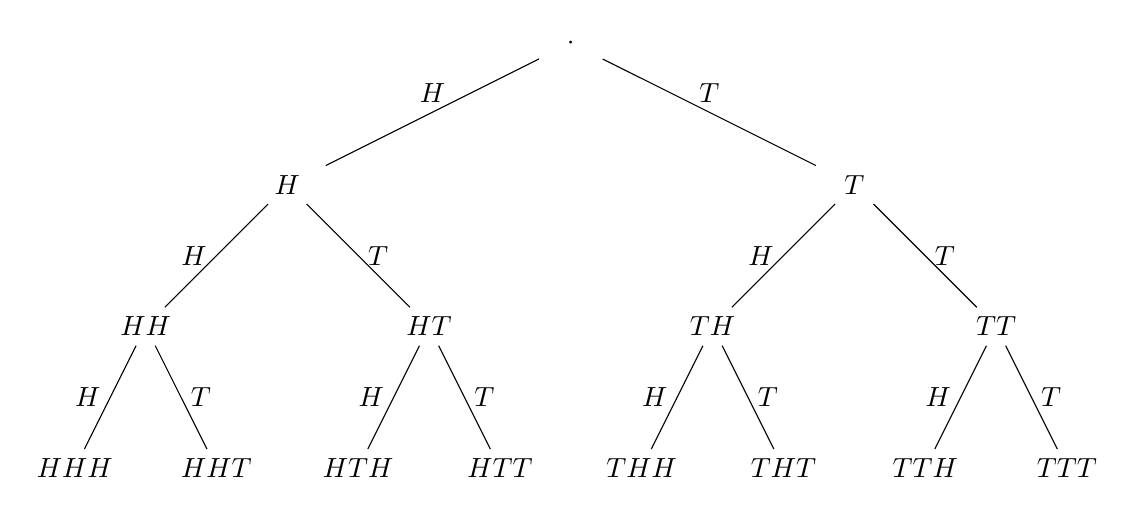
\begin{tikzpicture}[scale=.9]
            \tikzstyle{level 1}=[level distance=2cm, sibling distance=8cm]
            \tikzstyle{level 2}=[level distance=2cm, sibling distance=4cm]
            \tikzstyle{level 3}=[level distance=2cm, sibling distance=2cm]
            \tikzstyle{pause} = [text width=4em, text centered]
            \tikzstyle{end} = []

            \node [pause] {$\cdot$}
            child {
                    node [pause] {$H$}
                    child {
                            node [pause] {$HH$}
                            child {
                                    node [end] {$HHH$}
                                    edge from parent
                                    node [left] {$H$}
                                }
                            child {
                                    node [end] {$HHT$}
                                    edge from parent
                                    node [right] {$T$}
                                }
                            edge from parent
                            node [left] {$H$}
                        }
                    child {
                            node [pause] {$HT$}
                            child {
                                    node [end] {$HTH$}
                                    edge from parent
                                    node [left] {$H$}
                                }
                            child {
                                    node [end] {$HTT$}
                                    edge from parent
                                    node [right] {$T$}
                                }
                            edge from parent
                            node [right] {$T$}
                        }
                    edge from parent
                    node [above] {$H$}
                }
            child {
                    node [pause] {$T$}
                    child {
                            node [pause] {$TH$}
                            child {
                                    node [end] {$THH$}
                                    edge from parent
                                    node [left] {$H$}
                                }
                            child {
                                    node [end] {$THT$}
                                    edge from parent
                                    node [right] {$T$}
                                }
                            edge from parent
                            node [left] {$H$}
                        }
                    child {
                            node [pause] {$TT$}
                            child {
                                    node [end] {$TTH$}
                                    edge from parent
                                    node [left] {$H$}
                                }
                            child {
                                    node [end] {$TTT$}
                                    edge from parent
                                    node [right] {$T$}
                                }
                            edge from parent
                            node [right] {$T$}
                        }
                    edge from parent
                    node [above] {$T$}
                };
        \end{tikzpicture}
    \end{center}
\end{solution}

\begin{example}\label{example_sample_space_rolling_two_dice}
    Two dice are rolled. Write the sample space.
\end{example}
\begin{solution}
    We assume one of the dice is red, and the other green. We have the following 36 possibilities.

    \begin{center}
        \begin{tabular}{cc|cccccc}
            \multicolumn{1}{c}{} & \multicolumn{6}{c}{Green}                                                 \\
            %\cline{2-7}
                                 &                           & 1     & 2     & 3     & 4     & 5     & 6     \\
            \cline{2-8}
                                 & 1                         & (1,1) & (1,2) & (1,3) & (1,4) & (1,5) & (1,6) \\
                                 & 2                         & (2,1) & (2,2) & (2,3) & (2,4) & (2,5) & (2,6) \\
            Red                  & 3                         & (3,1) & (3,2) & (3,3) & (3,4) & (3,5) & (3,6) \\
                                 & 4                         & (4,1) & (4,2) & (4,3) & (4,4) & (4,5) & (4,6) \\
                                 & 5                         & (5,1) & (5,2) & (5,3) & (5,4) & (5,5) & (5,6) \\
                                 & 6                         & (6,1) & (6,2) & (6,3) & (6,4) & (6,5) & (6,6) \\
        \end{tabular}
    \end{center}

    The entry (2, 5), for example, indicates that the red die shows a 2, and the green a 5.
\end{solution}

\begin{summarybox}{Probability}

    For a sample space $S$ and an outcome $A$ of $S$, the following two properties are satisfied.
    \begin{enumerate}
        \item If $A$ is an outcome of a sample space, then the probability of $A$, denoted by $P(A)$, is between $0$ and $1$, inclusive.
              \[ 0 \leq P(A) \leq 1 \]
        \item The sum of the probabilities of all the outcomes in $S$ equals $1$.
    \end{enumerate}
\end{summarybox}

The probability $P(A)$ of an event $A$ describes the chance or likelihood of that event occurring.
\begin{itemize}
    \item If $P(A) = 0$, event $A$ will almost surely not occur.
    \item If $P(A) = 1$, event $A$ will almost surely occur.
    \item If $P(A) = 0.5$, then event $A$ is equally likely to occur or not occur.
\end{itemize}

\begin{note}
    It seems strange to use the phrase \textbf{almost surely} in that sentence. It seems like an event with probability zero is just impossible, but almost surely has a precise mathematical meaning. It's a bit beyond this course to explain, but we're going to try anyways. Suppose that you're throwing a dart at a dart board. The proability of hitting any single point is zero, but you've probably seen a dart hit a dart board, so it does happen. If you tried to hit the exact center of the board we'd expect it to take infinite time, but it's not impossible. In practice, we'd have a lot of trouble actually locating the exact center of the board because the markings on our measuring devices aren't thin enough\dots
\end{note}

%TODO make a little game with a pendulum that the student could play with here?

For example, if we toss a fair coin that is equally likely to land on heads or tails, then $P(\text{Head}) = 0.50$. If the weather forecast says there is a $70\%$ chance of rain today, then $P(\text{Rain}) = 0.70$, indicating it is more likely to rain than to not rain.

\begin{example}
    One 6 sided die is rolled once. Find the probability that the result is greater than 4.
\end{example}
\begin{solution}
    The sample space consists of the following six possibilities in set \( S \): \( S = \{1,2,3,4,5,6\} \)

    Let \( E \) be the event that the number rolled is greater than four: \( E = \{5,6\} \)

    Therefore, the probability of \( E \) is:
    \[ P(E) = \frac{2}{6} \text{ or } \frac{1}{3}. \]
\end{solution}


\begin{example}
    If two dice, one red and one green, are rolled, find the probability that the red die shows a 3 and the green shows a six.
\end{example}
\begin{solution}
    Since two dice are rolled, there are 36 possibilities. The probability of each outcome, listed in Example \ref{example_sample_space_rolling_two_dice}, is equally likely.

    Since \( (3, 6) \) is one such outcome, the probability of obtaining \( (3, 6) \) is \( \frac{1}{36} \).


\end{solution}

The example we just considered consisted of only one outcome of the sample space. We are often interested in finding probabilities of several outcomes represented by an event. An event is a subset of a sample space. If an event consists of only one outcome, it is called a simple event.

\begin{example}
    If two dice are rolled, find the probability that the sum of the faces of the dice is 7.
\end{example}
\begin{solution}
    Let \( E \) represent the event that the sum of the faces of two dice is 7.

    The possible cases for the sum to be equal to 7 are: \( (1, 6) \), \( (2,5) \), \( (3, 4) \), \( (4, 3) \), \( (5, 2) \), and \( (6, 1) \), so event \( E \) is
    \[ E = \{ (1, 6), (2,5), (3, 4), (4, 3), (5, 2), (6, 1) \} \]

    \begin{center}
        \begin{tabular}{c|cccccc}
              & 1             & 2             & 3             & 4             & 5             & 6             \\
            1 & (1,1)         & (1,2)         & (1,3)         & (1,4)         & (1,5)         & \boxed{(1,6)} \\
            2 & (2,1)         & (2,2)         & (2,3)         & (2,4)         & \boxed{(2,5)} & (2,6)         \\
            3 & (3,1)         & (3,2)         & (3,3)         & \boxed{(3,4)} & (3,5)         & (3,6)         \\
            4 & (4,1)         & (4,2)         & \boxed{(4,3)} & (4,4)         & (4,5)         & (4,6)         \\
            5 & (5,1)         & \boxed{(5,2)} & (5,3)         & (5,4)         & (5,5)         & (5,6)         \\
            6 & \boxed{(6,1)} & (6,2)         & (6,3)         & (6,4)         & (6,5)         & (6,6)         \\
        \end{tabular}
    \end{center}

    The probability of the event \( E \) is
    \[ P(E) = \frac{6}{36} \text{ or } \frac{1}{6}. \]
\end{solution}

\begin{example}
    A jar contains 3 red, 4 white, and 3 blue marbles. If a marble is chosen at random, what is the probability that the marble is a red marble or a blue marble?
\end{example}
\begin{solution}
    We assume the marbles are \( r_1, r_2, r_3 \) for red, \( w_1, w_2, w_3, w_4 \) for white, and \( b_1, b_2, b_3 \) for blue. Let the event \( C \) represent that the marble is red or blue.

    The sample space \( S \) is \{ \( r_1, r_2, r_3, w_1, w_2, w_3, w_4, b_1, b_2, b_3 \)\}

    And the event \( C \) = \{ \( r_1, r_2, r_3, b_1, b_2, b_3\) \}

    Therefore, the probability of \( C \),
    \[ P(C) = \frac{6}{10} \text{ or } \frac{3}{5}. \]
\end{solution}

\begin{example}\label{example_three_labeled_marbles_without_replacement_equal_5}
    A jar contains three marbles numbered 1, 2, and 3. If two marbles are drawn without replacement, what is the probability that the sum of the numbers is 5?
\end{example}
\begin{solution}
    Note, the two marbles in this example are drawn consecutively without replacement. That means that after a marble is drawn it is not replaced in the jar, and therefore is no longer available to select on the second draw.

    Since two marbles are drawn without replacement, the sample space consists of the following six possibilities.
    \[ S = \{ (1, 2), (1, 3), (2, 1), (2, 3), (3, 1), (3, 2) \} \]

    Note that \( (1,1), (2,2) \) and \( (3,3) \) are not listed in the sample space. These outcomes are not possible when drawing without replacement, because once the first marble is drawn but not replaced into the jar, that marble is not available in the jar to be selected again on the second draw.

    Let the event \( E \) represent that the sum of the numbers is five. Then
    \[ E = \{ (2, 3), (3, 2) \} \]

    Therefore, the probability of \( E \) is
    \[ P(E) = \frac{2}{6} \text{ or } \frac{1}{3}. \]
\end{solution}

\begin{example}\label{example_three_labeled_marbles_without_replacement_at_least_4}
    A jar contains three marbles numbered 1, 2, and 3. If two marbles are drawn without replacement, what is the probability that the sum of the numbers is at least 4?
\end{example}
\begin{solution}
    The sample space, as in Example \ref{example_three_labeled_marbles_without_replacement_equal_5}, consists of the following six possibilities.
    \[ S = \{ (1, 2), (1, 3), (2, 1), (2, 3), (3, 1), (3, 2) \} \]

    Let the event \( F \) represent that the sum of the numbers is at least four. Then
    \[ F = \{ (1, 3), (3, 1), (2, 3), (3, 2) \} \]

    Therefore, the probability of \( F \) is
    \[ P(F) = \frac{4}{6} \text{ or } \frac{2}{3}. \]
\end{solution}

\begin{example}\label{example_three_labeled_marbles_with_replacement_equal_5}
    A jar contains three marbles numbered 1, 2, and 3. If two marbles are drawn with replacement, what is the probability that the sum of the numbers is 5?
\end{example}
\begin{solution}
    When two marbles are drawn with replacement, the sample space consists of the following nine possibilities.
    \[ S = \{(1,1), (1, 2), (1, 3), (2, 1), (2, 2), (2, 3), (3, 1), (3, 2), (3,3)\} \]

    Let the event \( E \) represent that the sum of the numbers is five. Then
    \[ E = \{(2, 3), (3, 2)\} \]

    Therefore, the probability of \( E \) is
    \[ P(E) = \frac{2}{9} \]
\end{solution}

Note that in Example \ref{example_three_labeled_marbles_with_replacement_equal_5} when we selected marbles with replacement, the probability has changed from Example \ref{example_three_labeled_marbles_without_replacement_equal_5} where we selected marbles without replacement.

\begin{example}\label{example_three_labeled_marbles_with_replacement_at_least_4}
    A jar contains three marbles numbered 1, 2, and 3. If two marbles are drawn with replacement, what is the probability that the sum of the numbers is at least 4?
\end{example}
\begin{solution}
    The sample space when drawing with replacement consists of the following nine possibilities.
    \[ S = \{(1,1), (1, 2), (1, 3), (2, 1), (2, 2), (2, 3), (3, 1), (3, 2), (3,3)\} \]

    Let the event \( F \) represent that the sum of the numbers is at least four. Then
    \[ F = \{(1, 3), (3, 1), (2, 3), (3, 2), (2,2), (3,3)\} \]

    Therefore, the probability of \( F \) is
    \[ P(F) = \frac{6}{9} \text{ or } \frac{2}{3}. \]
\end{solution}

Note that in Example \ref{example_three_labeled_marbles_with_replacement_at_least_4} when we selected marbles with replacement, the probability is the same as in Example \ref{example_three_labeled_marbles_without_replacement_at_least_4} where we selected marbles without replacement.

Thus sampling with or without replacement MAY change the probabilities, but may not, depending on the situation in the particular problem under consideration.  We'll re-examine the concepts of sampling with and without replacement in Section \ref{section_probability_tree_and_combinations}.

